% Generated by book/tools/notebook_to_tex.py. Do not edit by hand.

\chapter[BERT 이진 분류: Sigmoid (BCE)]{BERT 이진 분류: Sigmoid (BCE)}

\markboth{BERT 이진 분류: Sigmoid (BCE)}{BERT 이진 분류: Sigmoid (BCE)}

\chaptermeta{10_bert_binary_sigmoid/10_bert_binary_sigmoid.ipynb}{https://colab.research.google.com/github/yoon-gu/neuqes-101/blob/master/10_bert_binary_sigmoid/10_bert_binary_sigmoid.ipynb}{num\_labels=1, sigmoid, BCEWithLogitsLoss 방식의 BERT 이진 분류}



\index{1BERT binary classification@BERT binary classification}

\index{1sigmoid@sigmoid}

\index{1BCEWithLogitsLoss@BCEWithLogitsLoss}

\index{1num labels 1@num\_labels=1}

\index{1multi label classification@multi\_label\_classification}

\index{1binary threshold@binary threshold}

\index{1ROC AUC@ROC AUC}

\index{1precision recall fscore support@precision\_recall\_fscore\_support}

\index{1prediction cache@prediction cache}

\index{0이진 분류@이진 분류}

\index{0시그모이드@시그모이드}

\index{0이진 교차 엔트로피@이진 교차 엔트로피}

\index{0확률 임계값@확률 임계값}

\index{0예측 저장@예측 저장}

\index{1AUC@AUC}

\index{1problem type multi label classification@problem\_type="multi\_label\_classification"}

\index{1sigmoid probability@sigmoid probability}

\index{1threshold 0 5@threshold=0.5}

\index{1roc auc score@roc\_auc\_score}

\index{1seaborn kdeplot@seaborn.kdeplot}

\index{1probability distribution@probability distribution}

\index{1positive class@positive class}

\index{1negative class@negative class}

\index{0확률 분포@확률 분포}

\index{0양성 클래스@양성 클래스}

\index{0음성 클래스@음성 클래스}

\index{0결과 캐시@결과 캐시}



\section{변화추적표}

\begin{booktable}{10장 변화추적표}{tab:ch10-01}
\begin{adjustbox}{max width=\textwidth}
\begin{tabular}{@{}lllllll@{}}
\toprule
Ch & 모델 & 토크나이저 & 데이터 & Output Head & Activation & Loss \\
\midrule

3 & \inlinecode{LogisticRegression()} & \inlinecode{TfidfVectorizer()} & Yelp 이진화 & (1차원) & sigmoid & \inlinecode{BCEWithLogitsLoss} \\
4 & \inlinecode{LogisticRegression(multi\_class="multinomial")} & \inlinecode{TfidfVectorizer()} & Yelp 이진화 (3장과 동일) & (2차원) & softmax & \inlinecode{CrossEntropyLoss} \\
9 & DistilBERT 파인튜닝 & \inlinecode{AutoTokenizer.from\_pretrained(...)} & Yelp (별점 1-5) & \inlinecode{Linear(H,\ 1)} & 없음 & \inlinecode{MSELoss} \\
\textbf{10 ← 여기} & DistilBERT 파인튜닝 & \inlinecode{AutoTokenizer.from\_pretrained(...)} & Yelp 이진화 & \textbf{\inlinecode{Linear(H,\ 1)}} & \textbf{sigmoid} & \textbf{\inlinecode{BCEWithLogitsLoss}} \\
11 (다음) & DistilBERT 파인튜닝 & 같음 & Yelp 이진화 & \inlinecode{Linear(H,\ 2)} & softmax & \inlinecode{CrossEntropyLoss} \\
\bottomrule
\end{tabular}
\end{adjustbox}
\end{booktable}

전체 20장 표는 \href{https://github.com/yoon-gu/neuqes-101\#챕터별-변화추적표}{루트 README.md}를 참고하세요.



\section{변경점: 9장 대비}

\begin{booktable}{10장 변경점 요약}{tab:ch10-02}
\begin{adjustbox}{max width=\textwidth}
\begin{tabular}{@{}lll@{}}
\toprule
축 & 9장 & 10장 \\
\midrule

Task & 회귀 & \textbf{이진 분류 (방식 A)} \\
\inlinecode{num\_labels} & 1 & \textbf{1} (그대로) \\
\inlinecode{problem\_type} & \inlinecode{"regression"} & \textbf{\inlinecode{"multi\_label\_classification"}} ← BCE 자동 적용 트릭 \\
Activation & 없음 & \textbf{sigmoid} (output head는 1차원, 학습 시 logit이 sigmoid 통과 후 BCE) \\
Loss & \inlinecode{MSELoss} & \textbf{\inlinecode{BCEWithLogitsLoss}} \\
라벨 & float (1-5) 별점 & \textbf{float {[}0.0 또는 1.0{]}} (multi-hot 1차원 벡터로 둠) \\
데이터 & Yelp 별점 1-5 & \textbf{Yelp 이진화} (4-5 → 1, 1-2 → 0, 3 제외) \\
\bottomrule
\end{tabular}
\end{adjustbox}
\end{booktable}

\subsection{\texorpdfstring{\inlinecode{num\_labels=1} + \inlinecode{problem\_type="multi\_label\_classification"} 의 트릭}{num\_labels=1 + problem\_type=“multi\_label\_classification” 의 트릭}}

\inlinecode{Trainer} 의 자동 loss 매핑은 이렇게 작동합니다 (\href{../09_bert_regression/09_bert_regression.ipynb}{9장에서 본 표}).

\begin{booktable}{10장 num\_labels=1 + problem\_type=“multi\_label\_classification” 의 트릭 표}{tab:ch10-03}
\begin{adjustbox}{max width=\textwidth}
\begin{tabular}{@{}llll@{}}
\toprule
\inlinecode{problem\_type} & 자동 적용 loss & num\_labels & 라벨 형식 \\
\midrule

\inlinecode{"regression"} & \inlinecode{MSELoss} & 보통 1 & float \\
\inlinecode{"single\_label\_classification"} & \inlinecode{CrossEntropyLoss} & K (≥2) & int 인덱스 \\
\inlinecode{"multi\_label\_classification"} & \textbf{\inlinecode{BCEWithLogitsLoss}} & K (≥1) & \textbf{multi-hot float} \\
\bottomrule
\end{tabular}
\end{adjustbox}
\end{booktable}

방식 A는 \emph{binary 분류이지만 num\_labels=1} 형태를 유지해야 합니다. 그러려면 \inlinecode{multi\_label\_classification} 으로 두어 BCE를 적용시키되, \emph{num\_labels=1짜리 multi-label} 즉 라벨을 길이 1짜리 multi-hot 벡터(\texttt{{[}0.0{]}} 또는 \texttt{{[}1.0{]}})로 만들면 됩니다. 이게 sklearn \inlinecode{LogisticRegression()} 의 sigmoid+BCE와 정확히 같은 셋업입니다.



\section{\texorpdfstring{손실 노트}{손실 노트}}

수식과 직관은 3장에서 봤습니다.

\begin{equation}
\label{eq:ch10-01}
L = -\frac{1}{N}\sum_{i=1}^{N}\left[\,y_i \log \hat p_i + (1 - y_i)\log(1 - \hat p_i)\,\right]
\end{equation}

식~\eqref{eq:ch10-01}은 정답 라벨과 예측 확률 사이의 Binary Cross-Entropy를 정의합니다.

이 장에서 새로운 점:

\begin{enumerate}
\def\labelenumi{\arabic{enumi}.}
\tightlist
\item
  \textbf{모델이 BERT} 라 logit \(z = w^\top h_{[CLS]} + b\) 의 \emph{분포 표현 \(h_{[CLS]}\)} 가 768차원 hidden state를 압축한 결과입니다 (sklearn TF-IDF 입력보다 풍부).
\item
  \inlinecode{BCEWithLogits} 의 \emph{Logits} --- 모델 마지막 단의 raw 점수에 sigmoid를 따로 통과시키지 않고 BCE 안에서 한꺼번에 처리하기 때문에 \textbf{수치적으로 안정} 합니다.
\item
  \inlinecode{Trainer} 가 \inlinecode{problem\_type="multi\_label\_classification"} 만 보고 자동으로 BCE를 골라줍니다. 우리는 라벨을 \texttt{{[}0.0{]}} 또는 \texttt{{[}1.0{]}} float 형태로 두기만 하면 됩니다.
\end{enumerate}

\textbf{숫자로 감 잡기} --- 3장 표 그대로:

\begin{booktable}{10장 손실 노트 표}{tab:ch10-04}
\begin{adjustbox}{max width=\textwidth}
\begin{tabular}{@{}lll@{}}
\toprule
정답 \(y\) & 예측 확률 \(\hat p\) & 손실 \(-\log \hat p\) \\
\midrule

1 & 0.9 & 0.105 \\
1 & 0.5 & 0.693 \\
1 & 0.1 & \textbf{2.303} \\
\bottomrule
\end{tabular}
\end{adjustbox}
\end{booktable}

확률이 0에 가까울수록 손실이 로그 스케일로 폭증한다는 BCE의 성격은 sklearn에서든 BERT에서든 동일합니다. 다른 점은 \emph{어떻게 그 확률을 만드느냐} 입니다 --- sklearn은 단어 빈도, BERT는 attention으로 압축한 문장 표현.



\section{토크나이저 노트}

7-9장와 같은 \inlinecode{distilbert-base-uncased} WordPiece 토크나이저. 토크나이저·데이터 가공 파이프라인은 8장에서 익힌 패턴을 그대로 적용합니다.

\begin{previewBox}{미리보기}
\textbf{다음 장(11장)}: 같은 토크나이저, 같은 데이터, 같은 BERT 본체. 변하는 건 출력 헤드가 1차원에서 2차원으로 늘어나고 sigmoid가 softmax로 바뀐다는 점뿐입니다.
\end{previewBox}



\Needspace{8\baselineskip}
\begin{lstlisting}
!pip install -q transformers datasets
\end{lstlisting}

\begin{codeRead}
\textbf{1행}의 \inlinecode{!pip install -q transform...}에서는 Colab 실행에 필요한 패키지를 설치합니다.
\end{codeRead}



\Needspace{26\baselineskip}
\begin{lstlisting}
import warnings
warnings.filterwarnings("ignore")

import numpy as np
import pandas as pd
import matplotlib.pyplot as plt
import seaborn as sns
import torch
from datasets import load_dataset
from transformers import (
    AutoTokenizer, AutoModelForSequenceClassification,
    Trainer, TrainingArguments,
)
from sklearn.metrics import (
    accuracy_score, precision_recall_fscore_support,
    classification_report, roc_auc_score,
)

plt.rcParams["axes.unicode_minus"] = False

print(f"PyTorch:        {torch.__version__}")
print(f"CUDA available: {torch.cuda.is_available()}")
if torch.cuda.is_available():
    print(
        f"GPU:             "
        f"{torch.cuda.get_device_name(0)}"
    )
else:
    print(
        "Warning: CPU runtime — training will be very "
        "slow. Switch to T4 recommended."
    )
\end{lstlisting}

\begin{codeRead}
\inlinecode{numpy, pandas, matplotlib, PyTorch, datasets} 같은 주요 패키지를 불러옵니다.
\end{codeRead}



\textbf{baseline VRAM}:



\Needspace{8\baselineskip}
\begin{lstlisting}
!nvidia-smi
\end{lstlisting}

\begin{codeRead}
\textbf{1행}의 \inlinecode{!nvidia-smi}에서는 앞 단계에서 만든 값을 바탕으로 다음 계산을 수행합니다.
\end{codeRead}



\section{데이터 준비}

별점 4-5는 \inlinecode{1.0} (긍정), 1-2는 \inlinecode{0.0} (부정), 3은 제외. 라벨을 \emph{float 1차원 multi-hot 벡터} (\texttt{{[}0.0{]}} 또는 \texttt{{[}1.0{]}}) 형태로 둡니다 --- 이게 BCE를 자동 적용시키는 핵심 형식.



\Needspace{26\baselineskip}
\begin{lstlisting}
tokenizer = AutoTokenizer.from_pretrained("distilbert-base-uncased")

ds = load_dataset("yelp_review_full")
train_full = ds["train"].shuffle(seed=42).select(range(5000))
eval_full  = ds["test"].shuffle(seed=42).select(range(1000))

def to_binary(example):
    star = example["label"] + 1   # 0-4 → 1-5
    if star == 3:
        return False
    return True

def add_binary(batch):
    bins = []
    for lbl in batch["label"]:
        star = lbl + 1
        bins.append(1.0 if star >= 4 else 0.0)
    batch["binary"] = bins
    return batch

train_bin = train_full.filter(lambda x: (x["label"] + 1) != 3).map(add_binary, batched=True)
eval_bin  = eval_full.filter(lambda x:  (x["label"] + 1) != 3).map(add_binary, batched=True)

print(f"train (after excluding 3-star): {len(train_bin)}")
print(f"eval  (after excluding 3-star): {len(eval_bin)}")
print(
    f"train positive rate: "
    f"{sum(train_bin['binary']) / len(train_bin):.1%}"
)
\end{lstlisting}



\Needspace{26\baselineskip}
\begin{lstlisting}
def tokenize_fn(batch):
    out = tokenizer(
        batch["text"],
        truncation=True,
        max_length=128,
    )

    out["labels"] = [[float(b)] for b in batch["binary"]]
    return out

train_tok = train_bin.map(
    tokenize_fn,
    batched=True).remove_columns(["text", "label", "binary"],
)
eval_tok  = eval_bin.map(
    tokenize_fn,
    batched=True).remove_columns(["text", "label", "binary"],
)

print(train_tok)
print(
    f"\nFirst sample label: "
    f"{train_tok[0]['labels']}  (length-1 float vector)"
)
\end{lstlisting}



\section{모델 로드}

\inlinecode{num\_labels=1} + \inlinecode{problem\_type="multi\_label\_classification"} 이 핵심.



\Needspace{26\baselineskip}
\begin{lstlisting}
model = AutoModelForSequenceClassification.from_pretrained(
    "distilbert-base-uncased",
    num_labels=1,
    problem_type="multi_label_classification",
)

def param_summary(m):
    total     = sum(p.numel() for p in m.parameters())
    trainable = sum(p.numel() for p in m.parameters() if p.requires_grad)
    return total, trainable

total, trainable = param_summary(model)
print(
    f"Parameters:           {total:>13,}  ("
    f"{total/1e6:.1f} M)"
)
print(
    f"Trainable parameters: {trainable:>13,}  ("
    f"{trainable/total:.1%})"
)
print(f"Classifier:           {model.classifier}")
print(
    f"problem_type:         "
    f"{model.config.problem_type}"
)
\end{lstlisting}



\Needspace{8\baselineskip}
\begin{lstlisting}
!nvidia-smi
\end{lstlisting}



\section{학습}

\inlinecode{compute\_metrics} 만 binary 분류용으로 새로 짭니다 --- sigmoid + threshold 0.5 로 0/1 예측을 만들고 accuracy/F1/AUC 계산.



\Needspace{25\baselineskip}
\begin{lstlisting}
def compute_metrics(eval_pred):
    logits, labels = eval_pred
    logits = logits.flatten()         # (B, 1) → (B,)
    labels = labels.flatten().astype(int)

    probs = 1.0 / (1.0 + np.exp(-logits))
    preds = (probs >= 0.5).astype(int)

    p, r, f1, _ = precision_recall_fscore_support(
        labels,
        preds,
        average="binary",
        zero_division=0,
    )
    return {
        "accuracy":  float(accuracy_score(labels, preds)),
        "precision": float(p),
        "recall":    float(r),
        "f1":        float(f1),
        "auc":       float(roc_auc_score(labels, probs)),
    }
\end{lstlisting}



\Needspace{26\baselineskip}
\begin{lstlisting}
training_args = TrainingArguments(
    output_dir="./ch10_output",
    num_train_epochs=2,
    per_device_train_batch_size=16,
    per_device_eval_batch_size=32,
    learning_rate=2e-5,
    fp16=True,
    eval_strategy="epoch",
    logging_steps=50,
    save_strategy="no",
    report_to="none",
    seed=42,
)

trainer = Trainer(
    model=model,
    args=training_args,
    train_dataset=train_tok,
    eval_dataset=eval_tok,
    processing_class=tokenizer,
    compute_metrics=compute_metrics,
)

train_result = trainer.train()
print(
    f"\nTraining done — mean train loss: "
    f"{train_result.training_loss:.4f}"
)
\end{lstlisting}



\Needspace{8\baselineskip}
\begin{lstlisting}
!nvidia-smi
\end{lstlisting}



\section{평가}

\inlinecode{Trainer.predict()} 로 logit을 받아 sigmoid를 통과시킨 확률 분포를 살펴봅니다.



\Needspace{9\baselineskip}
\begin{lstlisting}
eval_metrics = trainer.evaluate()
print("BERT method A evaluation:")
for k, v in eval_metrics.items():
    if k.startswith("eval_") and isinstance(v, float):
        print(f"  {k:>20}: {v:.4f}")
\end{lstlisting}



\Needspace{26\baselineskip}
\begin{lstlisting}
preds_output = trainer.predict(eval_tok)
logits = preds_output.predictions.flatten()
probs  = 1.0 / (1.0 + np.exp(-logits))
labels = preds_output.label_ids.flatten().astype(int)

print(
    f"Logit range: [{logits.min():.2f}, "
    f"{logits.max():.2f}]"
)
print(
    f"Prob range:  [{probs.min():.4f}, "
    f"{probs.max():.4f}]"
)
print(
    f"Positive prediction rate (prob >= 0.5): "
    f"{(probs >= 0.5).mean():.1%}"
)
print(f"\nFirst 5 samples:")
print(pd.DataFrame({
    "label": labels[:5],
    "logit": logits[:5].round(2),
    "prob":  probs[:5].round(4),
    "pred":  (probs[:5] >= 0.5).astype(int),
}).to_string(index=False))
\end{lstlisting}



\subsection{\texorpdfstring{확률 분포}{확률 분포}}

\inlinecode{seaborn.kdeplot} 으로 \emph{부드러운} 분포를 그립니다. histogram이 막대로 끊기는 반면 KDE는 연속 곡선이라 두 분포가 어디서 만나는지(=오분류 영역)가 한눈에 들어옵니다.

이 그림에서 봐야 할 세 가지:

\begin{itemize}
\tightlist
\item
  \textbf{양 끝 봉우리}: 학습이 잘 되면 라벨 0의 확률은 0 근처에, 라벨 1의 확률은 1 근처에 몰립니다 --- sigmoid가 큰 음수 logit을 0에, 큰 양수 logit을 1에 \emph{압착} 시키기 때문 (\(\sigma(z) = 1/(1+e^{-z})\) 의 양 극단 포화).
\item
  \textbf{0.5 근처의 교차 영역}: 두 곡선이 만나는 부분이 모델이 헷갈려하는 샘플들. 면적이 작을수록 분리가 잘 된 것.
\item
  \textbf{반대쪽 꼬리}: 라벨 0인데 확률 1쪽에, 라벨 1인데 확률 0쪽에 잡히는 작은 봉우리는 \emph{오분류}. 이 두 꼬리가 학습 손실(BCE)이 가장 크게 잡히는 영역.
\end{itemize}



\Needspace{21\baselineskip}
\begin{lstlisting}
sns.set_theme(style="whitegrid", context="talk")

df = pd.DataFrame({"prob": probs, "logit": logits, "label": labels})
PAL = {0: "#5B8DEF", 1: "#F47272"}

fig, ax = plt.subplots(figsize=(9, 5))
sns.kdeplot(
    data=df, x="prob", hue="label",
    fill=True, common_norm=False, alpha=0.5,
    palette=PAL, clip=(0, 1), ax=ax,
)
ax.axvline(0.5, color="black", lw=1.2, ls="--", alpha=0.7)
ax.set_title("Method A — Probability Distribution by Actual Label")
ax.set_xlabel("Predicted probability  P(y=1)")
ax.set_ylabel("Density")
plt.tight_layout()
plt.show()
\end{lstlisting}

\begin{bookfigurelabel}[htbp]{방식 A의 sigmoid 확률 분포}{fig:ch10-probability-kde}
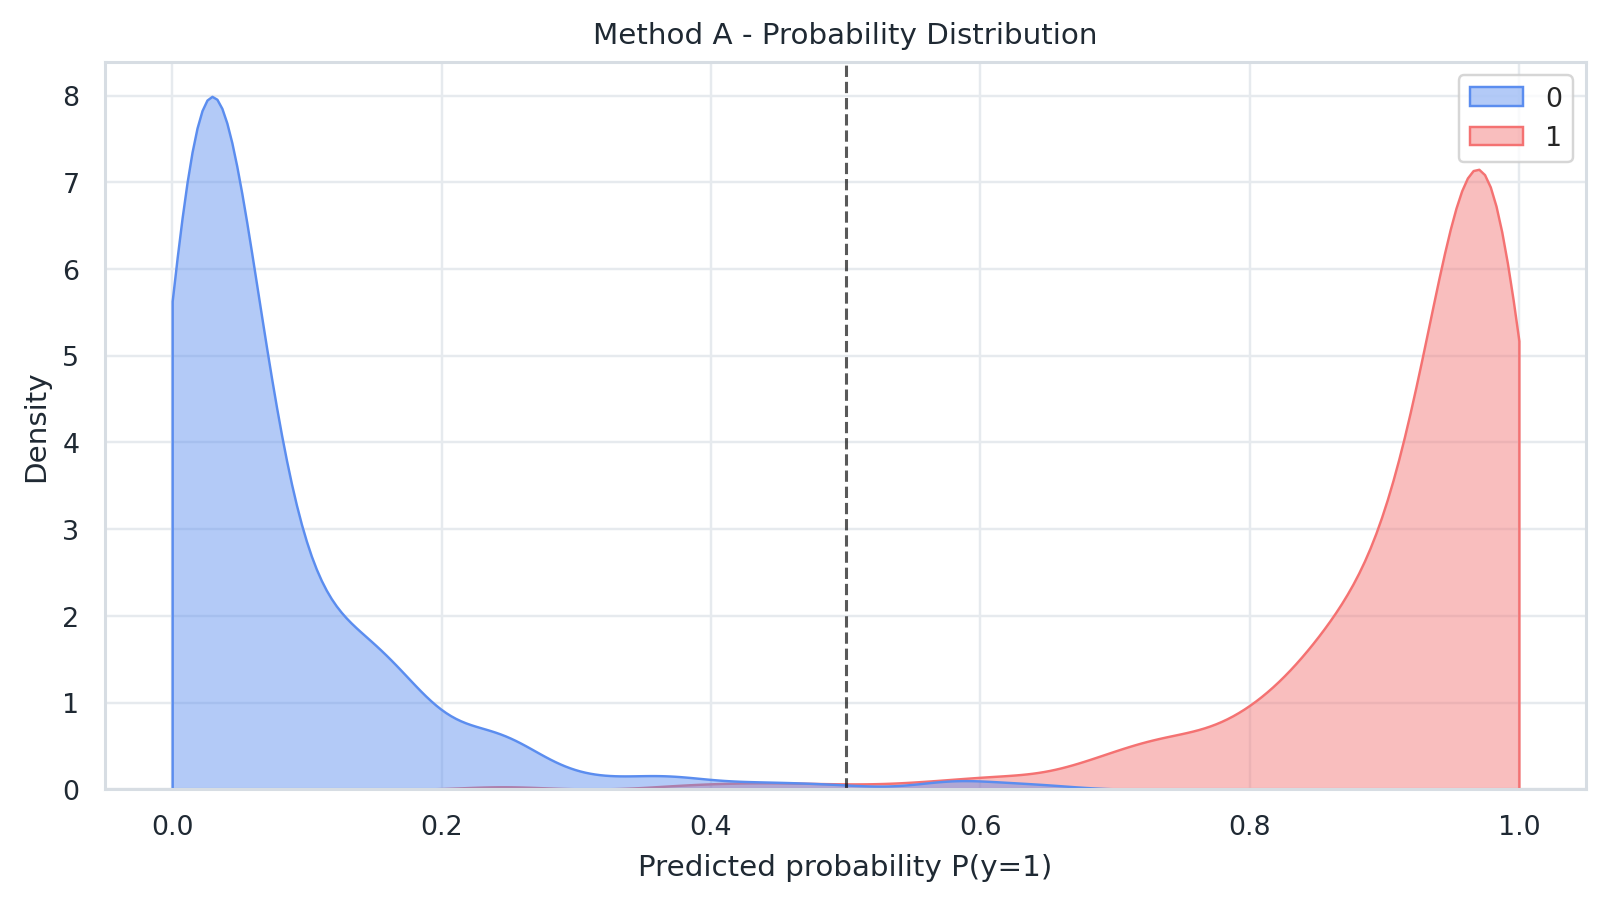
\includegraphics[width=0.88\linewidth]{assets/figures/ch10_probability_kde.png}
\end{bookfigurelabel}



\textbf{설명 --- 왜 양 끝이 솟아 있나?} sigmoid는 logit이 ±5만 넘어가도 거의 0 또는 1로 수렴합니다 (\(\sigma(5) \approx 0.993\), \(\sigma(-5) \approx 0.007\)). BERT가 학습 후 어느 정도 자신감을 갖게 되면 logit이 ±5-10 범위로 뻗어 나가고, 결과적으로 확률 공간에서는 \textbf{양 끝에 압착된 U자 분포}가 나옵니다. 가운데(0.3-0.7)는 모델이 \emph{판단을 망설이는} 샘플 --- 진짜 어려운 케이스이거나 라벨 노이즈일 가능성이 큽니다.

\textbf{\inlinecode{common\_norm=False} 의 의미}: 라벨별로 \emph{각자} 적분이 1이 되도록 정규화. 이렇게 해야 라벨 0 샘플 수와 라벨 1 샘플 수가 다를 때도 \emph{분포의 모양} 만 비교됩니다 (개수 차이는 빠짐).



\subsection{\texorpdfstring{로짓 분포}{로짓 분포}}

방금 본 확률 공간 그림은 사용자 눈에 보이는 결과지만, \textbf{\inlinecode{BCEWithLogitsLoss} 가 실제로 손실을 계산하는 자리} 는 \emph{logit 공간} 입니다 (\(z\), sigmoid를 통과하기 \emph{전}). 같은 데이터를 logit 축에서 다시 그려보면 사뭇 다른 풍경이 펼쳐집니다.

확률 공간(4-1)에서는 분포가 0과 1 양 끝에 \emph{압착}되어 안쪽 모양을 알 수 없었는데, logit 공간에서는 \textbf{두 개의 정규분포-비슷한 봉우리}가 결정 경계 \(z = 0\) 양옆에 일관되게 분리됩니다. 이게 BERT가 학습한 \emph{진짜 표상}에 더 가깝습니다.



\Needspace{17\baselineskip}
\begin{lstlisting}
fig, ax = plt.subplots(figsize=(9, 5))
sns.kdeplot(
    data=df, x="logit", hue="label",
    fill=True, common_norm=False, alpha=0.5,
    palette=PAL, ax=ax,
)
ax.axvline(0.0, color="black", lw=1.2, ls="--", alpha=0.7,
           label="decision boundary z=0")
ax.set_title("Method A — Logit Distribution (pre-sigmoid)")
ax.set_xlabel("Logit  z")
ax.set_ylabel("Density")
plt.tight_layout()
plt.show()
\end{lstlisting}

\begin{bookfigurelabel}[htbp]{방식 A의 sigmoid 이전 logit 분포}{fig:ch10-logit-kde}
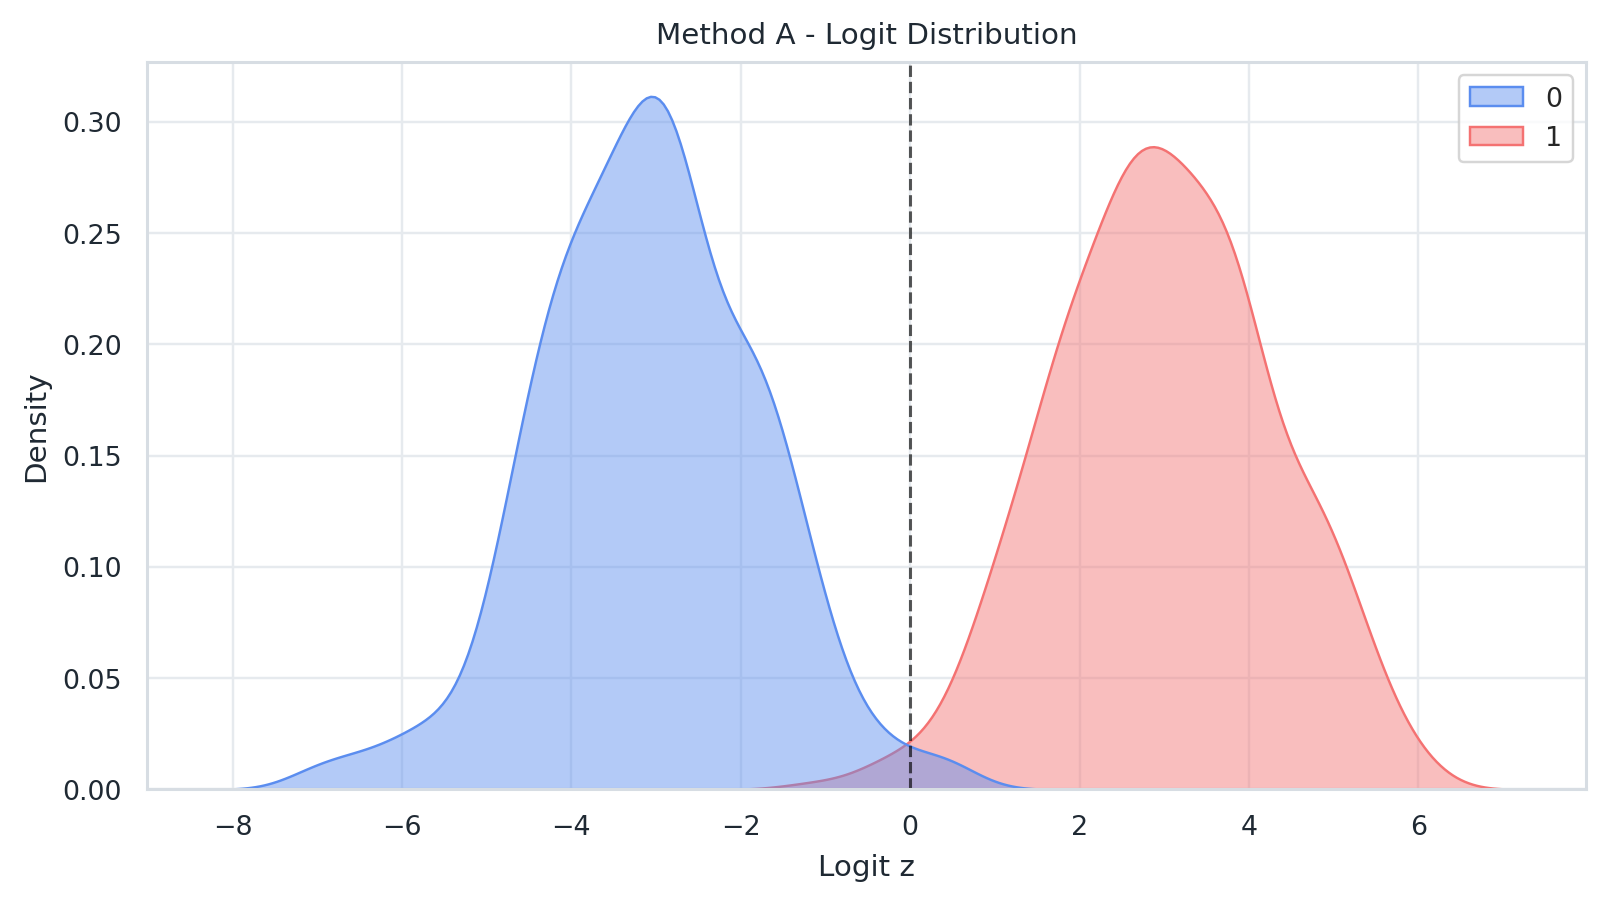
\includegraphics[width=0.88\linewidth]{assets/figures/ch10_logit_kde.png}
\end{bookfigurelabel}



\textbf{두 그림을 함께 보는 법 --- sigmoid가 한 일}

\begin{itemize}
\tightlist
\item
  확률 공간(4-1)의 \emph{양 끝 압착} 은 logit 공간(4-2)의 \emph{바깥쪽 꼬리} 에서 옵니다. logit이 +6 이든 +10 이든 sigmoid 통과 후엔 모두 0.99 이상이라 구분이 안 됨 --- 정보가 \emph{압축} 되는 것.
\item
  결정 경계는 두 그림 모두 \emph{같은 자리}: 확률에서 0.5, logit에서 0. 단지 좌표축이 다를 뿐.
\item
  두 봉우리의 \textbf{거리} 는 logit 공간에서만 의미가 있습니다. 거리가 멀수록 모델이 두 클래스를 자신 있게 구분하는 것. 확률 공간에서는 이 거리가 양 끝 압착 때문에 안 보입니다.
\end{itemize}

\textbf{왜 \inlinecode{BCEWithLogitsLoss} 인가} --- BCE를 \emph{확률} 위에서 계산하면 (\(p = \sigma(z)\)), \(\log p\) 와 \(\log(1-p)\) 가 양 극단에서 0에 매우 가까운 수가 되어 로그 안의 수치가 폭주합니다 (\inlinecode{log(0)} 발산). 반면 logit 위에서 직접 계산하면 (\(\text{BCE}(z, y) = \max(z, 0) - z y + \log(1 + e^{-\vert{}z\vert{}})\)) 로그-합-지수(log-sum-exp) 트릭으로 \textbf{수치적으로 안정}. 그래서 우리는 모델 출력 logit을 sigmoid 통과 \emph{없이} 그대로 \inlinecode{BCEWithLogitsLoss} 에 넣습니다.



\Needspace{9\baselineskip}
\begin{lstlisting}
print(classification_report(
    labels, (probs >= 0.5).astype(int),
    target_names=["negative", "positive"],
    digits=4,
))
\end{lstlisting}



\section{결과 저장}

다음 장 11장에서 같은 데이터에 \emph{방식 B} (softmax+CE)로 학습한 뒤 \emph{이번 방식 A} 의 결과와 비교합니다. 평가 지표와 확률 예측을 디스크에 저장해 두면 비교가 깔끔해집니다.



\Needspace{26\baselineskip}
\begin{lstlisting}
import json, os

os.makedirs("./shared_binary_results", exist_ok=True)

np.save(
    "./shared_binary_results/method_a_probs.npy",
    probs,
)
np.save(
    "./shared_binary_results/method_a_labels.npy",
    labels,
)

method_a_summary = {
    "method": "A (sigmoid + BCE, num_labels=1)",
    "metrics": {
        k.replace("eval_", ""): v
        for k, v in eval_metrics.items()
        if k.startswith("eval_") and isinstance(v, float)
    },
}
with open("./shared_binary_results/method_a_summary.json", "w") as f:
    json.dump(method_a_summary, f, indent=2)

print("Saved: ./shared_binary_results/")
for f in sorted(os.listdir("./shared_binary_results")):
    size_kb = os.path.getsize(f"./shared_binary_results/{f}") / 1024
    print(f"  {f}  ({size_kb:.1f} KB)")
\end{lstlisting}



\textbf{참고}: Colab은 세션이 끝나면 \inlinecode{./shared\_binary\_results/} 가 사라집니다. \emph{Drive에 보존} 하려면 다음과 같이 마운트.

\Needspace{11\baselineskip}
\begin{lstlisting}
from google.colab import drive
drive.mount("/content/drive")
import shutil
shutil.copytree(
    "./shared_binary_results",
    "/content/drive/MyDrive/neuqes-101/shared_binary_results",
)
\end{lstlisting}

11장 노트북은 같은 세션에서 이어 돌리거나, 같은 데이터·seed·모델로 다시 학습해서 결과를 만든 뒤 비교합니다.



\section{이 장에 등장한 라이브러리·함수}

\begin{booktable}{10장 새로 등장한 라이브러리}{tab:ch10-05}
\begin{adjustbox}{max width=\textwidth}
\begin{tabular}{@{}lll@{}}
\toprule
이름 & 한 줄 설명 & 다음 장에서 \\
\midrule

\inlinecode{AutoModelForSequenceClassification(num\_labels=1,\ problem\_type="multi\_label\_classification")} & num\_labels=1 + multi\_label로 BCE 자동 매핑 & 12-13장에서 multi-hot 라벨로 재사용 \\
\inlinecode{sklearn.metrics.precision\_recall\_fscore\_support} & 이진 분류 지표 한 묶음 & 11·15장·17에서 동일 \\
\inlinecode{sklearn.metrics.roc\_auc\_score} & AUC 계산 (확률 임계값 무관) & 분류 장마다 사용 \\
\inlinecode{numpy\ 1/(1+exp(-x))} & sigmoid 직접 구현 (모델 logit → 확률) & 7장에서 본 동일 패턴 \\
\inlinecode{seaborn.kdeplot(...,\ hue=,\ fill=True,\ common\_norm=False)} & 라벨별 부드러운 분포를 \emph{각자} 정규화해 모양만 비교 & 분류 장마다 동일 패턴으로 재등장 \\
\bottomrule
\end{tabular}
\end{adjustbox}
\end{booktable}



\section{체크포인트 질문}

\begin{enumerate}
\def\labelenumi{\arabic{enumi}.}
\tightlist
\item
  \inlinecode{num\_labels=1} 인데 왜 \inlinecode{problem\_type="single\_label\_classification"} 이 아닌 \inlinecode{"multi\_label\_classification"} 으로 두나요?
\item
  \inlinecode{BCEWithLogitsLoss} 의 \emph{Logits} 가 의미하는 바는? sigmoid를 따로 적용하지 않는 이유는?
\item
  학습 후 \emph{확률 공간} 에서 라벨별 분포가 양 끝에 압착되는 이유는? 같은 분포를 \emph{logit 공간} 에서 보면 무엇이 달라지나요? (4-1, 4-2 그래프 비교)
\item
  같은 binary 분류를 sklearn \inlinecode{LogisticRegression()} 으로 풀 때(3장)와 BERT로 풀 때(10장), accuracy 차이가 어디서 오나요?
\end{enumerate}



\section{FAQ}

\begin{faqBox}{Q1. (실무) \inlinecode{num\_labels=1} 일 때 \inlinecode{problem\_type="single\_label\_classification"} 으로 두면 안 되나요?}

안 됩니다. \inlinecode{single\_label\_classification} 은 CrossEntropyLoss를 적용하는데, CE는 \texttt{num\_labels\ \textgreater{}=\ 2} 를 가정합니다. \inlinecode{num\_labels=1} 로 두고 CE를 적용하면 logit이 단 하나라 softmax가 항상 1을 출력하고, loss가 항상 0이 되어 학습이 안 됩니다.

방식 A의 정수 라벨이 0/1 두 개이지만 \emph{출력은 1차원 logit} 이므로 --- 이 형태를 \inlinecode{Trainer} 가 이해하게 하려면 \inlinecode{multi\_label\_classification} 으로 두어야 BCE가 자동 적용됩니다.

\end{faqBox}

\begin{faqBox}{Q2. (이론) 라벨을 길이 1 multi-hot 벡터(\texttt{{[}0.0{]}}, \texttt{{[}1.0{]}})로 두는 이유는?}

\inlinecode{BCEWithLogitsLoss} 가 \emph{logits 와 같은 shape의 float 텐서} 를 라벨로 받기 때문입니다.

\Needspace{7\baselineskip}
\begin{lstlisting}
# logits.shape = (batch, num_labels=1)

loss = BCEWithLogitsLoss()(logits, labels)
\end{lstlisting}

라벨을 scalar(\inlinecode{float(b)})로 두면 batching 시 shape가 (batch,)가 되어 (batch, 1) logits와 안 맞습니다. \texttt{{[}float(b){]}} 한 번 감싸 length-1 list로 두면 (batch, 1) shape이 자동으로 만들어집니다.

\end{faqBox}

\begin{faqBox}{Q3. (실무) \inlinecode{compute\_metrics} 의 \inlinecode{eval\_pred.predictions} 는 어떤 형태인가요?}

\inlinecode{AutoModelForSequenceClassification} 의 출력은 \emph{logits} 입니다 (sigmoid 적용 전).

\begin{itemize}
\tightlist
\item
  방식 A (이 장, num\_labels=1): shape \inlinecode{(batch,\ 1)}. flatten 후 sigmoid 적용 → 확률.
\item
  방식 B (11장, num\_labels=2): shape \inlinecode{(batch,\ 2)}. softmax 적용 → 두 확률.
\end{itemize}

\inlinecode{compute\_metrics} 안에서 우리가 sigmoid·argmax·threshold 같은 후처리를 직접 합니다.

\end{faqBox}

\begin{faqBox}{Q4. (이론) sklearn LogReg(3장)와 BERT(10장)의 accuracy 차이는 어디서?}

세 가지 layer에서 차이가 옵니다.

\begin{enumerate}
\def\labelenumi{\arabic{enumi}.}
\tightlist
\item
  \textbf{단어 표현}: TF-IDF는 단어 독립 벡터, BERT는 문맥 attention. \inlinecode{"not\ bad"} vs \inlinecode{"bad"} 구분이 BERT만 가능.
\item
  \textbf{모델 capacity}: TF-IDF + LogReg는 \textasciitilde10K개 가중치, BERT는 67M개. 표현력 6,700배 차이.
\item
  \textbf{사전학습}: BERT는 위키피디아·BookCorpus로 미리 학습돼 일반 언어 지식이 모델에 인코딩됨.
\end{enumerate}

다만 Yelp 별점 같은 \emph{단어 빈도} 가 강한 신호인 task는 sklearn도 90\% 이상 잘 맞춰서, 차이가 \emph{극적이지 않은} 경우도 있습니다. 차이가 명확히 드러나는 task는 부정·반어가 많은 sentiment 데이터(SST-2)나 NLI(자연어 추론)입니다.

\end{faqBox}

\begin{faqBox}{Q5. (실무) 같은 데이터로 두 번 학습하면 결과가 똑같나요?}

\textbf{거의 같지만 미세한 차이가 있습니다}. 이유:

\begin{itemize}
\tightlist
\item
  random seed (\inlinecode{seed=42}) 고정해도 \emph{CUDA 비결정성} 이 남음 (cuDNN의 일부 알고리즘이 floating point 연산 순서를 비결정적으로 처리).
\item
  DataLoader의 shuffle, dropout, layer init은 seed로 통제되지만 GPU 부동소수 연산 자체가 결정적이지 않음.
\end{itemize}

완전히 결정적으로 만들려면 \inlinecode{torch.use\_deterministic\_algorithms(True)} 같은 옵션이 있지만 속도가 느려집니다. 실무에선 \emph{seed 여러 개로 학습 후 평균} 이 일반적.

\end{faqBox}

\begin{faqBox}{Q6. (실무) 학습 도중 학습률을 어떻게 조정하나요?}

\inlinecode{Trainer} 는 기본으로 \emph{linear warmup → linear decay} 스케줄러를 적용합니다. \inlinecode{lr\_scheduler\_type} 으로 바꿀 수 있습니다.

\Needspace{9\baselineskip}
\begin{lstlisting}
TrainingArguments(
    ...,
    lr_scheduler_type="cosine",
    warmup_ratio=0.1,
)
\end{lstlisting}

작은 데이터·짧은 학습이면 default linear가 무난. 학습 중 LR을 직접 모니터링하려면 \inlinecode{report\_to="wandb"} 같은 트래커 필수.
\end{faqBox}



\section{오류 실험 (선택)}

다음 코드를 돌려보면 어떤 에러가 날까요?

\Needspace{12\baselineskip}
\begin{lstlisting}
def tokenize_wrong(batch):
    out = tokenizer(
        batch["text"],
        truncation=True,
        max_length=128,
    )
    out["labels"] = [float(b) for b in batch["binary"]]
    return out
\end{lstlisting}

힌트: \inlinecode{BCEWithLogitsLoss(logits,\ labels)} 에서 logits.shape는 \inlinecode{(B,\ 1)} 인데 labels.shape가 \inlinecode{(B,)} 가 되어 broadcasting 또는 shape mismatch 에러가 납니다. 정확히 어떤 메시지가 뜨는지 확인해 보세요.



\begin{previewBox}{미리보기: 다음 장}

\textbf{11장. BERT 이진 분류 B (Softmax \& CE)}

\begin{itemize}
\tightlist
\item
  같은 Yelp 이진화 데이터, 같은 BERT 본체
\item
  \inlinecode{num\_labels=2} + \inlinecode{problem\_type="single\_label\_classification"} (BERT 표준)
\item
  Activation은 softmax, Loss는 \inlinecode{CrossEntropyLoss}
\item
  학습 후 \emph{방식 A의 저장된 결과} 와 직접 비교 --- 두 방식이 거의 같은 확률 분포를 만들어내는지 확인 (4장의 sklearn 동등성을 BERT에서 다시)
\item
  학습된 가중치 비교, 두 방식의 prediction agreement 측정
\end{itemize}
\end{previewBox}
